\documentclass[aspectratio=169]{beamer}
\usepackage[english]{babel}
\usepackage{booktabs,listings}
\usepackage[T1]{fontenc}
\usepackage[utf8]{inputenc}

\usetheme[slogan=english,mathfont=serif]{NTNU}

\newcommand{\mean}[1]{\left\{\!\!\left\{#1\right\}\!\!\right\}}
\newcommand{\jump}[1]{\left[\!\!\left[ #1 \right]\!\!\right]}
\newcommand{\abs}[1]{\left\lvert #1 \right\rvert}

	\title[Your Short Title]{ Cut Finite Element Method for the Cahn-Hilliard Equation}
	\subtitle{And why it is quite cool stuff}
	\author{Isak Hammer}
	\date{\today}

\begin{document}
	\maketitle

	\section{Introduction}\label{sec:introduction}

Cell membranes are the foundation of the origin of life, but also linked to the dynamics of virus al infections and genetic mutations since it controls what substances that can exit or enter the cell \cite{ hurley2010membrane}. In fact, a good
understanding of the cell membrane is important of engineering proteins to manipulate various intracellular processes in living systems \cite{rojas1998genetic}.

One of the primary components of the cell membranes are lipids which serve many different functions. A key function is that it is consisting of a bilayer of lipids which controls the structural rigidity and the fluidity of the membrane. Thus, elastic
bending forces, temperature and diffusion is essential on how a cell membrane will evolve \cite{udo97,neidleman87}.


\subsection{Elastic bending energy on evolving surfaces}%
\label{sub:willmore_flow}

Assuming that the system is a single-phase system, i.e., the lipids are uniformly distributed, can the elastic bending energy be modelled using the Canham-Helrich energy functional \cite{helfrich1973elastic, wang08, udo97}. Let us denote $b_{b},
b_{k}$ and $H_{0}$ as parameters based on physical models, then can the energy functional be denoted as,
\begin{equation}
\label{eq:CH}
\mathcal{E} _{CH}\left( \Gamma\left( t \right)   \right) =   \int_{\Gamma  }^{}  b_{b} \left( H- H_{0} \right) ^{2} + b_{k} K
.\end{equation}
Here is $H =  \kappa_1 + \kappa_2 $ denoted as the mean curvature and $K = \kappa_1 \kappa_2$ as the gaussian curvature with respectively and $\kappa_1$ and $\kappa_2$ as principal curvatures. $\Gamma \left( t
\right) = \Gamma  $ is here an evolving surface in $\mathbb{R} ^3$, for more info see section \ref{sec:background}.  Using the Gauss-Bonnet theorem can it be shown that the problem above is equivalent to the so-called Willmore energy
functional \cite{montiel2009curves, willmore1996riemannian},

\begin{equation}
\label{eq:WE}
\mathcal{E} _{W} \left( \Gamma\left( t \right)   \right) = \int_{\Gamma  }^{} \frac{1}{2} H ^2
.\end{equation}

This is a well known problem in the mathematical community \cite{ topping2000towards, marques2014willmore,link2013gradient,kuwert2012willmore}. In fact, it is a mathematical tool used to study the geometry of surfaces because it can be used to study
the diffeomorphism from a initial surface to a minimal energy configuration, which are surfaces with the least possible area for a given boundary. This is important in many areas of mathematics, including differential geometry, topology and mathematical physics \cite{koerber2021area,jakob2022singularities, rupp21}.

It has been established many numerical methods for for shape optimization problems \cite{sokolowski1992introduction,ito2008variational}, evolving surface partial differential equations (PDE) \cite{dziuk2013finite, dziuk2007finite,
binz2022convergent, barrett2007parametric, barrett2007variational, kovacs2019convergent, lehrenfeld2018stabilized} and specific
algorithms for the Willmore energy problem \eqref{eq:WE} \cite{palmurella2022parametric, dziuk2008computational, bonito2010parametric,  kovacs2021convergent, hu2022evolving}.

\subsection{Two-phase separation modelling on predefined evolving surfaces }%
\label{sub:two_phase_seperation_modelling_on_surfaces_}

It also turns out that the lipids often accumulate into so-called lipid rafts which serves as a rigid platform for proteins with special properties such as intracellular trafficking of lipids and lipid-anchored proteins \cite{ miller2020divide}. Modelling of
lipid rafts formation can be modelled as a two-phase separation problem based on minimization of the Ginzburg-Landau energy functional \cite{yushutin19},
\begin{equation}
\label{eq:GL}
\mathcal{E}_{GL}  \left( c   \right) = \int_{\Gamma\left(t  \right)   }^{}\Psi \left( c \right) + \frac{\gamma}{2} \left\lvert \nabla c \right\rvert^{2} ,
\end{equation}
which describes the chemical energy for a concentration $c: \Gamma\left( t \right)  \times \left[ 0,T \right] \mapsto  \left[ 0,1 \right]  $. Here is $ \Psi \left( c \right): \mathbb{R} \mapsto \mathbb{R} $ denoted as a nonlinear scalar chemical potential function. Keep in mind that unlike
the Willmore energy functional \eqref{eq:WE}, where the $\Gamma\left( t \right)  $ is determined by the elastic properties, should the energy functional \eqref{eq:GL} be interpreted as a chemical diffusion problem a predefined evolving domain $\Gamma \left( t \right) $.
Usually is this problem solved by deriving equivalent variants of partial differential equations (PDE) such as Allen-Cahn equation (or Cahn-Hilliard equation if the total concentration is globally conserved) on evolving domains. For further details,
see \cite{yushutin19,
udo97, ratz16,Gera2017, caetano21, elliott2015evolving}.

\subsection{Multiphysics problems on evolving surfaces}%

Ultimately will the cell membrane consists of interaction several kinds of physics (temperature, elasticity, chemical diffusion, internal fluid pressure etc.) \cite{udo97}. Hence, being able to model several processes may give unforeseen results.

An interesting example is to couple the energy functionals \eqref{eq:GL}  and \eqref{eq:CH}, since the lipid-rafts formation is said to change the elasticity properties of the membrane, may be a good model for how cell membranes evolve to specific shapes or execute cell division. One way
to couple the energy functionals is to let the parameters $b_{b}, b_{k}$ and $ H_{0} $ be some function of the time dependent concentration $c$, i.e.,
\[
    \begin{split}
        \mathcal{E}_{CHGL} \left( \Gamma\left( t \right) ,c\left( t \right)    \right) =  & \int_{\Gamma  }^{}  b_{b}\left( c \right)  \left( H- H_{0}\left( c \right)  \right) ^{2}  \\
        & + \int_{\Gamma   }^{} b_{k}\left( c \right)  K \\
        &+ \int_{\Gamma   }^{}\Psi \left( c \right) + \frac{\gamma}{2} \left\lvert \nabla c \right\rvert^{2} ,
    \end{split}
\]
For more information, see \cite{elliott2010surface}.

Recently have some authors also coupled diffusion processes and the so-called mean curvature energy, see \cite{burger2021interaction, elliott2022numerical}. It is well known that lipids travels
along the cell membrane in a fluidic manner, hence, it is also of interest to couple the Ginzburg-Landau energy functional \eqref{eq:GL} (or more specifically the Cahn-Hilliard equation) with the Navier-Stokes equation. Some methods has been proposed
methods for solving the problem on surfaces
and evolving surfaces, but it remains a field of active research \cite{olshanskii2022comparison}. As far as a author knows, coupling the Canham-Helrich energy functional \eqref{eq:CH}, Ginzburg-Landau energy functional \eqref{eq:GL}  and Navier-Stokes equation remains a open problem.

Some physical processes may require constant area and volume. This can simply be added by introducing respectively area and volume functionals, see \cite[Definition 2.5]{muller2013volume}.

Until now have all the models assumed that the membrane has no difference in internal and external pressure. As a matter of fact, osmotic pressure can be introduced by adding a energy functional using the van't Hoff formula. Let $V_{p}$ be the volume
of a closed evolving surface $\Gamma \left( t \right) $, we can then model the difference of internal and external pressure as,
\[
\Delta P \left( V_{p} \right) = P_{in} - P_{out} = iRT\left( \frac{n}{V_{p}} - \overline{c}  \right),
\]
where $i, R, T, \overline{c} $ and $n$ are the van't Hoff index, ideal gass constant, temperature , ambient molar concentration and molar amount of the enclosed solute. Then the energy
functional have the form,
\[
\mathcal{E} _{p}\left( \Gamma    \right)  = \int_{\Gamma   }^{   } \Delta P\left( V_{p} \right) ,
\]
For more information, see \cite{zhu2022mem3dg}.


\subsection{Outline of this report}%
\label{sub:outline_of_this_report}

The long-term goal would be to solve the multi-physics problems above. However, many of the problems above is fairly complicated to solve numerically and requires sophisticated techniques. Hence, in this report we focus on the latest research withing
the numerical methods of finding the minima of the energy functional \eqref{eq:WE}. However, we will first establish notation by including a section for definitions and important results from differential geometry and shape derivatives. We will then derive the
underlying dynamics system of evolutionary system dynamics using the gradient flow technique inspired by shape optimization methods based on the work done in \cite{ dougan2012first}. Lastly, we will establish the numerical methods of the system
dynamics by applying recent methods using an evolutionary surface finite element method (FEM) \cite{kovacs2021convergent, hu2022evolving}.




	\begin{frame}{Contents}
        \textbf{Plan for today}
        \begin{enumerate}
        \item Introduction - 2 min
        \item The Cahn Hilliard Equation - 3 min
        \item Introduction to CutFEM - 4 min
        \item Results (hehehe) - 2 min
        \item Questions - 5 min
        \end{enumerate}

        \begin{block}{My goal is to give you a taste of modern finite element methods!}

    \end{block}

	\end{frame}
	% % intro


\newpage
\section{Finite Element Method}%
\label{sec:finite_element_method}


\begin{frame}{}
        \begin{block}{Finite Element Methods!}
            \begin{itemize}
                \item To simplify will I only consider Poisson equation $ \Delta u =f $
                    \begin{itemize}
                        \item However, same ideas applies to Navier-Stokes and Cahn-Hilliard
                    \end{itemize}
                \item But to tell the story we need to do math
                    \begin{itemize}
                        \item Notation, inverse inequalities, variational forms, domains etc
                        \item \textbf{I will skip a lot of details,} but still promote the main ideas.
                    \end{itemize}
            \end{itemize}
        \end{block}
\end{frame}

\begin{frame}{}
        \begin{block}{We start with finite difference}
            \begin{itemize}
                \item Then we gradually introduce flaws and problems!
            \end{itemize}
        \end{block}
\end{frame}

\begin{frame}{Poisson Problem}
    Let us define the physical domain $\Omega  \subset \mathbb{R} ^{2}$ and the scalar functions $f: \Omega  \to \mathbb{R}$ and $g: \Omega  \to \mathbb{R} $.
        \begin{block}{Poisson Problem}
  We define the strong formulation of the Possion problem to find a scalar solution
 $u:\Omega  \to \mathbb{R} $ s.t. \[
\begin{split}
    -\Delta u &= f \quad  \text{in }\Omega  \\
     u &= g  \quad \text{on } \Gamma      \\
\end{split} .
\]
        \end{block}
\end{frame}

\begin{frame}{}
        \begin{block}{Finite difference approach}
            \begin{itemize}
                \item Taylor expansion in $y$ and $x$ direction. \[
                        \begin{split}
                \Delta u & = u_{xx} + u_{yy} \\
                & \approx  \frac{u( x-h, y) - 2u( x,y) + u( x +h,y)   }{h^2} + \frac{u( x, y-h) - 2u( x,y) + u( x,y +h)   }{h^2}
                        \end{split}
                \]
            \item Works very well for perfectly square domains
                \begin{figure}
                    \centering
                    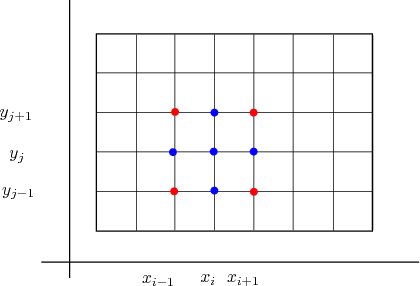
\includegraphics[width=0.35 \textwidth]{figures/fdm.png}
                \end{figure}
            \end{itemize}
        \end{block}
\end{frame}

\begin{frame}{}
        \begin{block}{Finite difference approach}
            \begin{itemize}
            \item Can be very messy for unstructured mesh!
                \begin{figure}
                    \centering
                    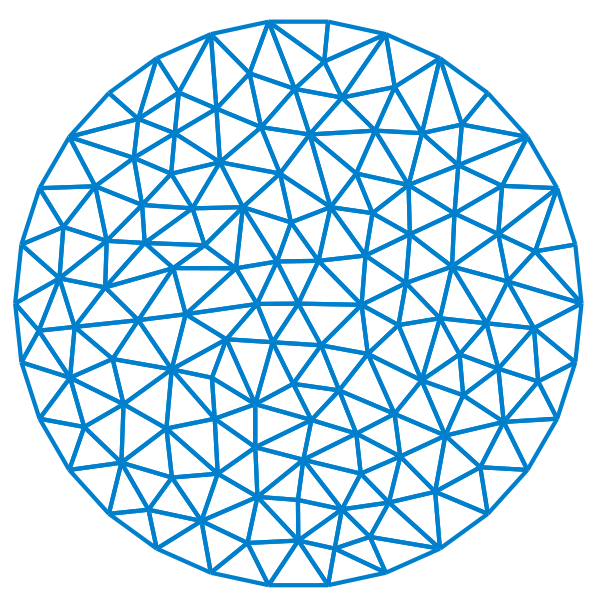
\includegraphics[width=0.35 \textwidth]{figures/triangulation.png}
                \end{figure}
            \item It does exists methods for handling nodes on these domains.
                \begin{itemize}
                    \item The implementation can be very messy
                    \item Does not scale that well as far as I know.
                \end{itemize}
            \end{itemize}
        \end{block}
\end{frame}


\begin{frame}{Finite element method}
        \begin{block}{Finite element approach for triangulations}
            \begin{enumerate}
                \item We want to write the problem on a equivalent integral form.
                \item Introduce so-called test functions space
                \item Introduce a discrete polynomial space as an approximation space.
            \end{enumerate}
        \end{block}
\end{frame}

\begin{frame}{Finite element method}

        \begin{block}{Let us introduce some notation}
            \begin{itemize}
                \item
                 Function spaces
                    \begin{equation*}
                        \begin{split}
                        L^{2}( \Omega  ) & = \left\{ f: \Omega \mapsto \mathbb{R}  \mid \int_{\Omega }^{} \left\lvert f \right\rvert ^{2} d \Omega  < \infty  \right\} \\
                        H^{1}( \Omega  ) & = \left\{ u \in L^{2}\left( \Omega  \right)  \text{ and }  \nabla  u \in L^{2}\left( \Omega  \right)   \right\}.
                        \end{split}
                    .\end{equation*}

                \item Essentially is $L^2( \Omega ) $ the space of all integrable functions.
                    \begin{itemize}
                        \item \textbf{Example:} $ \int_{-1}^{1} (\frac{1}{x}) dx  $ is not $L^2(\left[ -1,1 \right] )$  integrable. \\
                        \item \textbf{Example:} $ \int_{2}^{3} (\frac{1}{x}) dx  $ is $L^2(\left[ 2,3 \right] )$  integrable. \\
                    \end{itemize}


                \item $H^{1}( \Omega )$ is the space off all functions where both the function and its first derivative is integrable.
            \end{itemize}

        \end{block}
\end{frame}


\begin{frame}{Finite element method}

        \begin{block}{Norms and inner products}
            \begin{itemize}
                \item For $u ,v \in L^2( \Omega )  $ we define  \[
                        \begin{split}
\| u \|_{  \Omega   }^{  } & = \| u \|_{ L^{2}\left( \Omega  \right)  }^{  }   = \left( \int_{\Omega }^{} \left\lvert u \right\rvert ^{2} dx  \right) ^{\frac{1}{2}} \\
\left( u,v \right) _{\Omega } & = \left( u,v \right) _{L^2\left( \Omega  \right) } = \int_{\Omega }^{} u  v dx. \\
                        \end{split}
                    \]
                \item  For $u,v \in H^1( \Omega ) $ we define \[
                    \begin{split}
\| u \|_{ H^{1}\left( \Omega  \right)  }^{  }  & =  \| u \|_{ \Omega } +\| \nabla u \|_{ \Omega }    , \\
\left( u,v \right) _{H^{1}( \Omega )  } & = \left( u,v \right) _{\Omega  } + \left( \nabla u, \nabla v \right) _{\Omega  }
                    \end{split} .
                    \]
            \end{itemize}

        \end{block}

\end{frame}


\begin{frame}{Finite element method}
        \begin{block}{Writing the Poission problem on an integral form   }
            \begin{enumerate}
                \item We extent the definitions for the boundary conditions s.t.
                    \begin{itemize}
                        \item $H^{1}_{0} = \left\{ v \in H^{1 }( \Omega )   \mid  v = 0 \text{ on } \Gamma   \right\} $
                        \item  $V_{g} = \left\{ v \in H^{1 }( \Omega )   \mid  u = g \text{ on }  \Gamma   \right\} $
                    \end{itemize}
                    Notice that the boundary conditions is built in to the space!
                \item Let $u \in V_{g}$. If we multiply with a so-called test function $v \in H^{1}_{0}( \Omega ) $ and apply Greens theorem we get
                    \[
                - \int_\Omega  \Delta u v dx  = \int_\Omega  \nabla u \nabla v dx - \int_\Gamma \partial _{n} u v dx  =  \int_\Omega  \nabla u \nabla v dx
                    \]

                    We will use the following compact notation:
                    \[
                -( \Delta u, v) _{\Omega } = ( \nabla u, \nabla v)_{\Omega} - (\partial _{n} u, v )_{\Gamma }  =  ( \nabla u, \nabla v)_{\Omega}
                \]

            \end{enumerate}
        \end{block}
\end{frame}

\begin{frame}{Finite element method}
        \begin{block}{Writing the Poission problem on an integral form  }
             Let us denote a bilinear form and a linear form \[
            a( u,v)  := ( \nabla u,\nabla v)_{\Omega } \text{ and }  \quad l ( v) := ( f,v) _{\Omega  }
            \]
            The weak formulation of the Poisson problem is to find a $u \in V_{g}$ s.t. \[
            a( u,v) = l ( v) \quad  \forall v  \in  H^{1}_{0}( \Omega  )
            \]

        \end{block}

        How can we discretize the following function spaces?
\end{frame}

\begin{frame}{Abstract definition of a finite element}
    \begin{block}{}
    We define a element as the triple $(T, \mathcal{P}, \Sigma )$ where,
    \begin{itemize}
        \item $T$ is an triangle
        \item $\mathcal{P}^{k}( T)   $ is a finite polynomial basis $\left\{ \phi  \right\}_{i}^{n} $  of dimension $k$, also known as shape functions.
        \item $\Sigma $ is the dual of $\mathcal{P}^{k}( T)  $, that is, the set of linear forms $\left\{ \sigma _{i} \right\}_{i}^{n} $ with the mapping,
            \[
            \sigma _{i}:  \mathcal{P}^{k}( T) \to \mathbb{R} \quad  \text{ such that  } \quad   \sigma _{i}( \phi _{j})  = \delta _{ij}
            \]
            Also contains the DOFs or the coefficients in the polynom!
    \end{itemize}
    \end{block}

    \textbf{Example:} For $k=1$ the DOF in a triangle is one coefficient per mesh node, i.e., number of DOFs is $n = 3$.


\end{frame}

\begin{frame}{Finite element method}
    The absolute key idea of the finite element methods is the following; \\
    \begin{itemize}
        \item \textbf{ The goal is to approximate the (infinite dimensial) function space $H^{1}( \Omega ) $ with a finite dimensional polynomial space $\mathcal{P}^{k}( \Omega ) = span  \left\{ \phi_{1}, \ldots, \phi _{N}  \right\} $ of order $k$  }
    \end{itemize}

\end{frame}

\begin{frame}{Finite element method}
    To solve the Poisson problem using FEM we have the following discrete problem;

    \begin{block}{ Discrete Poisson problem }
    We want to find an $u_{h} \in V_{h} := \mathcal{P}^{k}( \Omega )  $ s.t. \[
    a( u_{h}, v_{h}) = l ( v_{h}) \quad  \forall v_{h} \in V_{h}
    \]
    \end{block}

\end{frame}

\begin{frame}{Finite element method}

    \begin{block}{ Constructing the linear system  }
        \begin{itemize}
            \item Since $v_{h}, u_{h} \in V_{h} := \mathcal{P}^{k}( \Omega )  $ can we write $u_{h} = \sum_{i=0}^{N} U_{i} \phi _{i} $ and $v_{h} = \sum_{i=0}^{N} U_{i} \phi _{i} $ with coefficients $\left\{ U_{i} \right\}_{i=0} ^{N} $ and $\left\{ V_{i} \right\}_{i=0} ^{N} $.
        \item Let us define a matrix $\left[ \mathcal{A}  \right] _{ji} = a( \phi_{i}, \phi _{j} ) $ and $\left[ F \right] _{j} = l( \phi _{j})   $.
        \end{itemize}
    \end{block}
    Thus, we have \[
    \sum_{i,j}^{N} V_{j} U_{i}\ a( \phi_{j}, \phi _{i} ) =  \sum_{j}^{N} V_{j}\ l(\phi _{j})     .
    \]
    Hence, we have the following equivalent linear system, that is \[
    \mathcal{A} U = F.
    \]
\end{frame}

\begin{frame}{Energy norm}

   We will now show requirements for uniqueness of numerical solution, but we need the so-called energy norm.

   \begin{block}{  }
    The energy norm  is denoted by  \[
    \| v \|_{a  }^{ 2 } = a( v,v)
    \]
    \end{block}



\end{frame}

\begin{frame}{Requirements for a well-posed problem}
    \begin{theorem}[ The (discrete) Lax-Milgram Theorem]
        Assume we have a general the bilinear form  $a_{h}: V_{h} \times V_{h} \to \mathbb{R}  $ and a bounded linear form $l_{h}: V_{h} \to \mathbb{R} $. If there exists some constants $C_{1} >0$ and $C_{2} >0$  such that;
        \begin{enumerate}
            \item The bilinear form is bounded,
                \[
                      \abs{a_{h}( v,w)  }    \le C_{1} \| v \|_{a_{h}  }^{  }  \| w \|_{a_{h}  }^{  } \quad \forall v,w  \in V_{h}.
                \]
            \item The bilinear form is coercive (one-to-one), \[
           a_{h}( v,v) \ge  C_{2} \| v \|_{ a_{h} }^{  2} \quad \forall v \in V_{h}.
            \]
        \end{enumerate}
        then it exists a unique discrete solution $u \in V_{h}$ s.t. \[
        a_{h}( u,v)  = l_{h}( v) \quad  \forall v \in V_{h}
        \]
    \end{theorem}


\end{frame}

\begin{frame}{Why is a well-posed problem so interesting?}
    \begin{block}{ Consequences of Lax Milgram }
    \begin{enumerate}
        \item The solution is accurate and reliable.
        \item The discrete problem converges when $h\to 0$
        \item Does not exists infinite solutions
        \item The problem is stable respect to small perturbation.
    \end{enumerate}

    \end{block}
    \begin{block}{Conclusion}
        \begin{itemize}
            \item Lax-Milgram very useful and rigour tool when developing new FEM schemes.
            \item Still hard to apply directly nonlinear problems, but we use it as a basis on simplified problems before we introduce nonlinear terms.
                \begin{enumerate}
                    \item Stokes equation vs Navier Stokes equation
                    \item Biharmonic equation vs Chan Hilliard equation
                \end{enumerate}
        \end{itemize}
    \end{block}

\end{frame}





	
\newpage
\section{Cut Finite Element method}%
\label{sec:cut_finite_element_method}

\begin{frame}{Classical Methods}

    \begin{block}{ What is the problem?  }
        \begin{itemize}
            \item It is suboptimal on moving domains $ \Omega ( t)  $ .
            \item And only works if $\Omega $ can be fully covered by by the mesh \[
            \Omega = \bigcup_i T_{i}
            \]
            Thus, cannot handle smooth boundaries.
        \end{itemize}
    \end{block}

\end{frame}

\begin{frame}{Great we have a solution}

    \begin{block}{ What is the problem?  }
        \begin{itemize}
            \item It is suboptimal on moving domains $ \Omega ( t)  $ .
            \item And only works if $\Omega $ can be fully covered by by the mesh \[
            \Omega = \bigcup_i T_{i}
            \]
            Thus, cannot handle smooth boundaries.
        \end{itemize}
    \end{block}
\end{frame}

\begin{frame}{}
    \begin{block}{ Moving Domains }
        \begin{itemize}
            \item Potentially very costly re-meshing procedures.
            \item Ill-conditioned if mesh is too bad
        \end{itemize}
                \begin{figure}
                    \centering
                    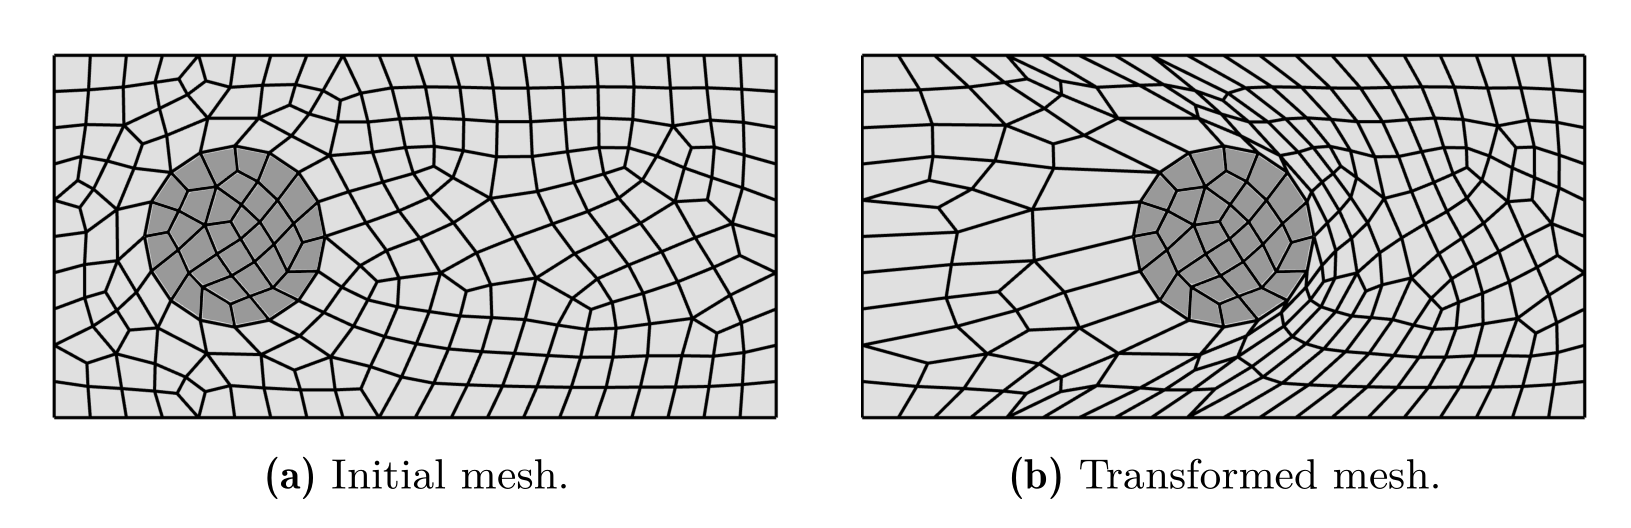
\includegraphics[width=0.95 \textwidth]{figures/transformed_mesh.png}
                \end{figure}
    \end{block}
\end{frame}


\begin{frame}{}

    \begin{block}{ Other problems of unstructured mesh }
        \begin{itemize}
            \item Unstructured mesh is difficult to parallelize
            \item Cannot handle smooth boundaries. Some application may actually require smooth boundaries (shape optimization etc).
        \end{itemize}
    \end{block}
    \begin{figure}
        \centering
        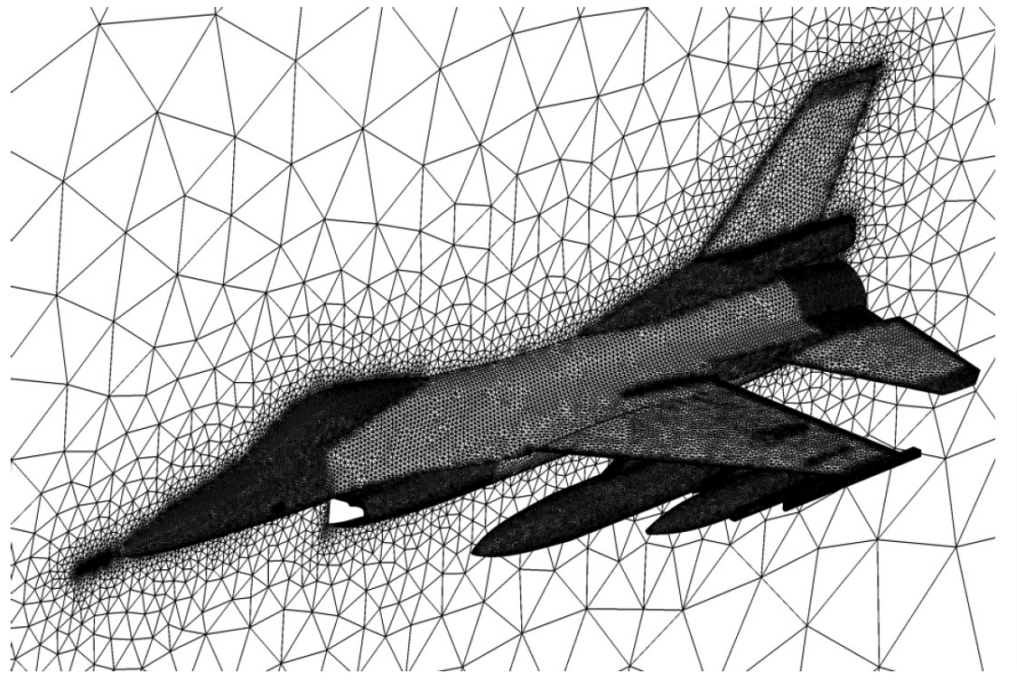
\includegraphics[width=0.45 \textwidth]{figures/unstructured_mesh_f16.png}
    \end{figure}
\end{frame}

\begin{frame}{Ways to solve this problem}
    \begin{itemize}
        \item Change the geometry.
            \begin{enumerate}
                \item Time-dependent mesh elements on moving domains.
                \item Delete and add nodes when necessary.
                \item Full re-mesh generation.
                \item Probably many more clever methods $\ldots$
            \end{enumerate}
        \item Utilize the geometry instead of modifying it
            \begin{enumerate}
                \item Method that can handle smooth boundaries.
                \item Do some smart transformations
            \end{enumerate}
    \end{itemize}
    \begin{block}{Question}
        \textbf{How do you approach this problem?}
    \end{block}

\end{frame}

\begin{frame}{Cut finite element method}
     Method to solve PDE's with moving domains on a unfitted mesh!
                \begin{figure}
                    \centering
                    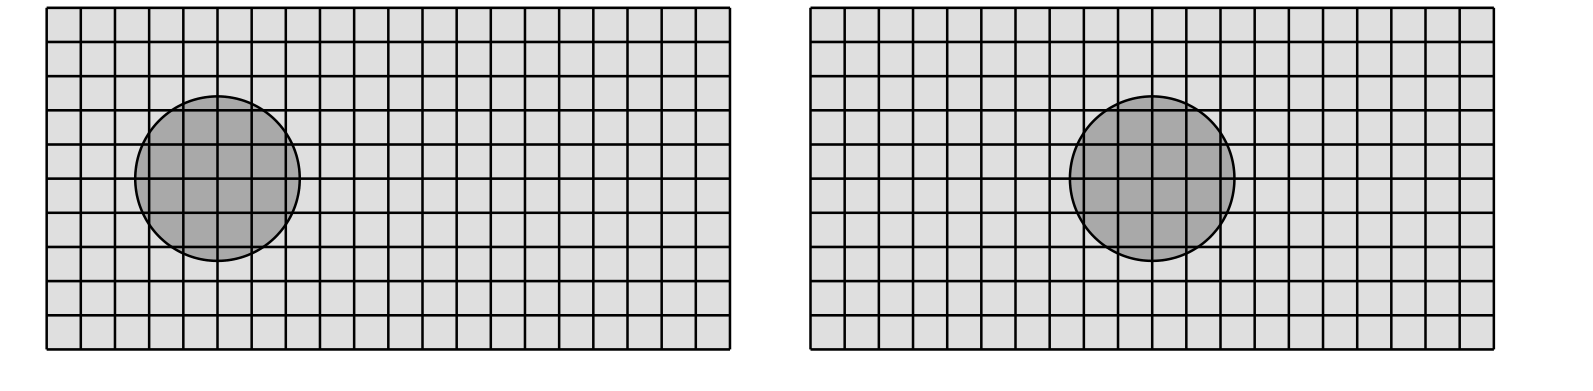
\includegraphics[width=0.95 \textwidth]{figures/transformed_mesh_unfitted.png}
                \end{figure}
    \begin{block}{  }
        \begin{itemize}
            \item Here we considering an smooth boundary $\Gamma $ in $C^2$
            \item No re-meshing on moving domains, only new configuration of cut cells.
            \item Potential to handle very complex geometries
        \end{itemize}
    \end{block}

\end{frame}

\begin{frame}{Example of complex domains}

        \begin{figure}
            \centering
            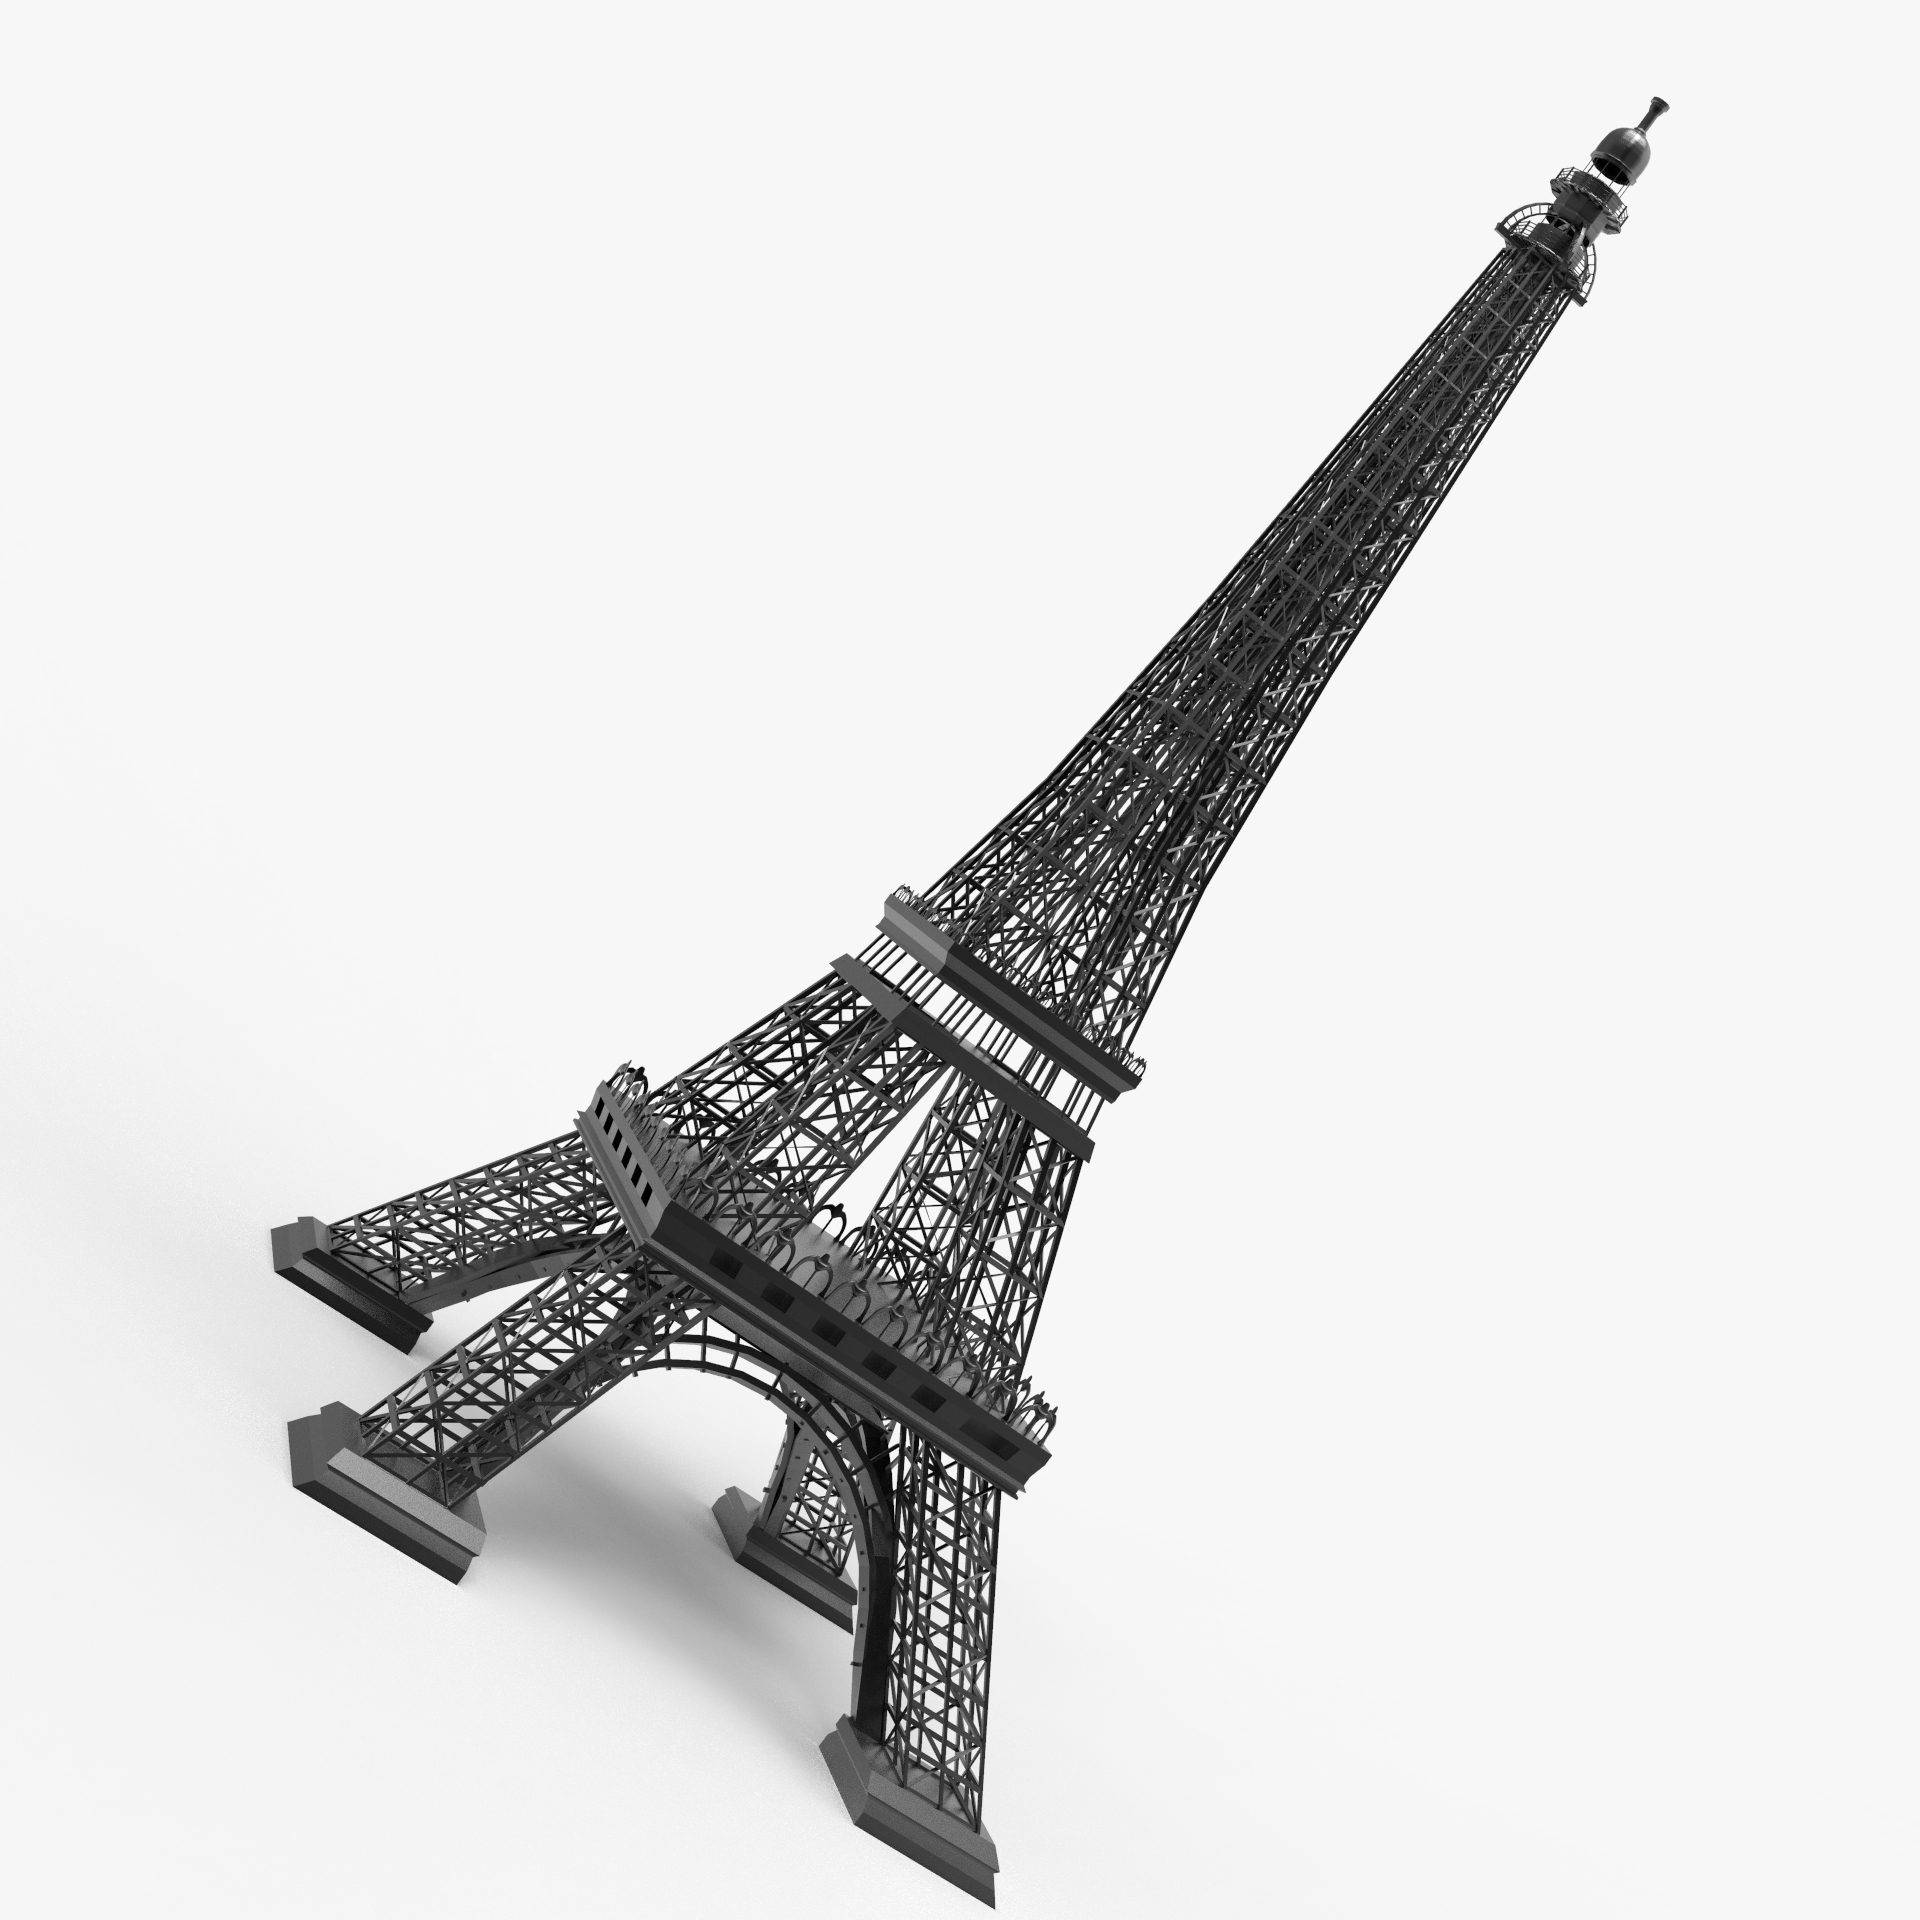
\includegraphics[width=6cm]{figures/eiffel_tower.jpg}
        \end{figure}

\end{frame}
\begin{frame}{Navier-Stokes on moving domains}

        \begin{figure}
            \centering
            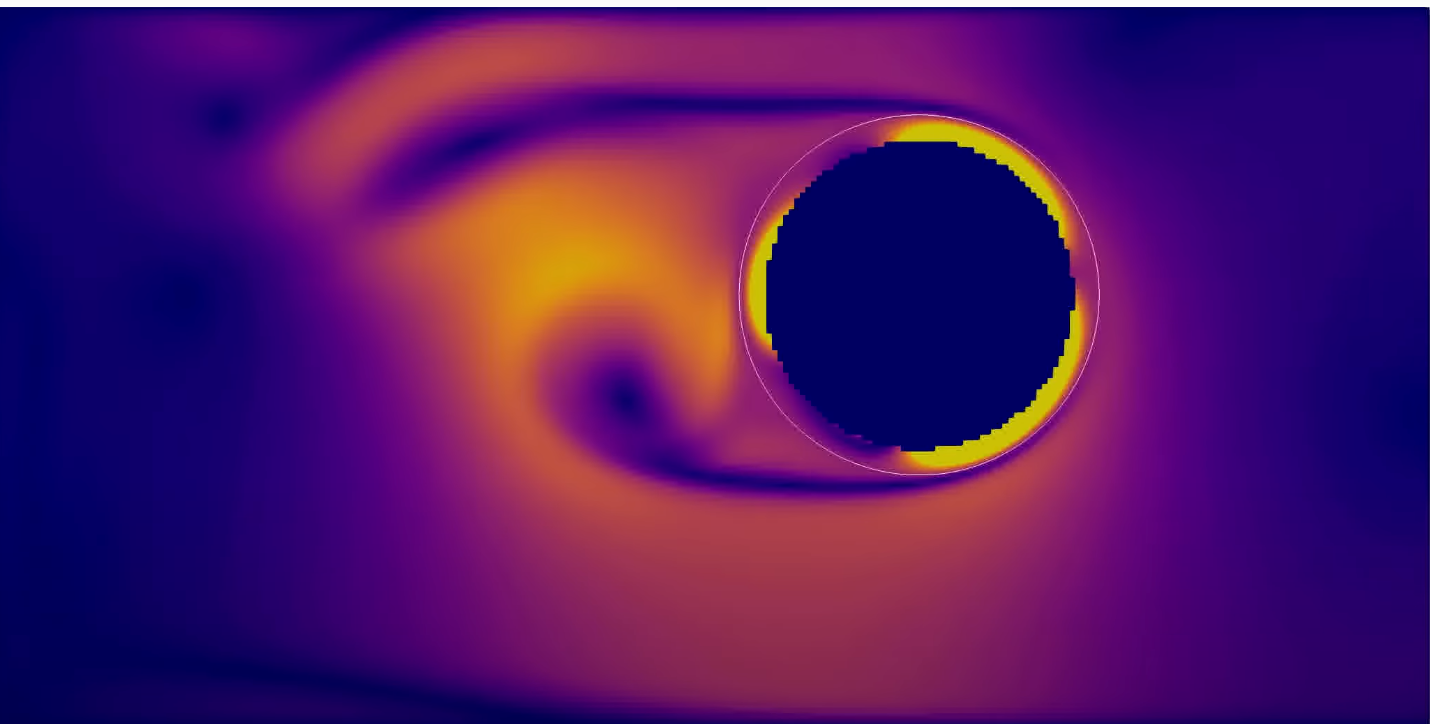
\includegraphics[width=8cm]{figures/navier_stokes.png}
        \end{figure}

    \href{https://www.youtube.com/watch?v=9dYdPOgPDUI&ab_channel=SigmundEggenHolm}{Link} to video
\end{frame}
\begin{frame}{Computational Domains}
    \begin{block}{}
        \begin{figure}
            \centering
            \parbox{5cm}{
                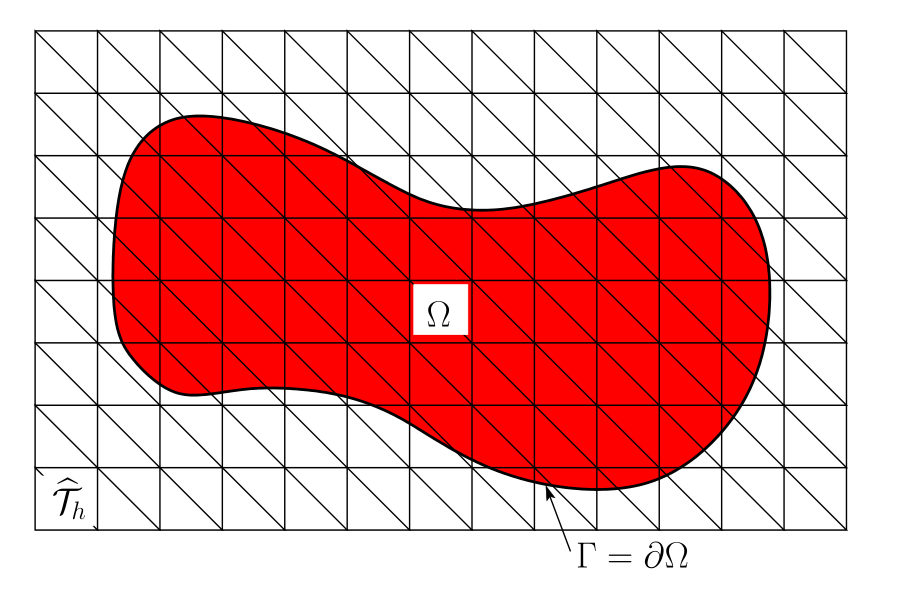
\includegraphics[width=4.5cm]{figures/physical_domain.png}
                \caption{Physical domain}
            \label{fig:2figsA}}
            \qquad
            \begin{minipage}{5cm}
                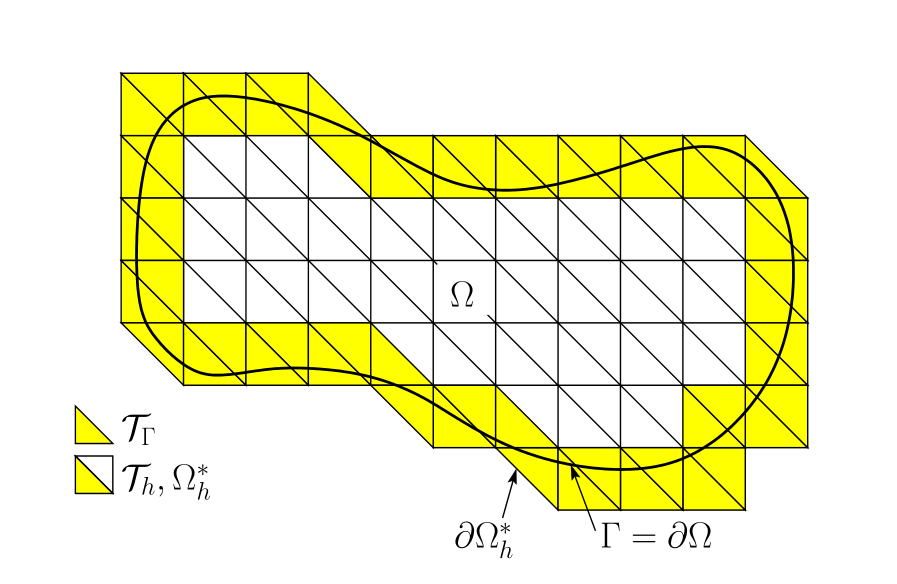
\includegraphics[width=4.5cm]{figures/minimal_subset.png}
                \caption{Cut cells}
                \label{fig:2figsB}
            \end{minipage}
        \end{figure}
        \begin{itemize}
            \item We define a background mesh $\widetilde{\mathcal{T} }_{h}$
            \item An active submesh $\mathcal{T} _{h} \subset \widetilde{\mathcal{T} _{h}}$ containing physical domain $\Omega $.
            \item Cut cells $ \mathcal{T} _{\Gamma} \subset \mathcal{T} _{h} $ is the mesh elements that intersects with the boundary $\Gamma  $.
        \end{itemize}
    \end{block}
\end{frame}

\begin{frame}{Constructing the method}
        \begin{columns}
        \begin{column}{0.5\textwidth}
        \begin{figure}
            \centering
            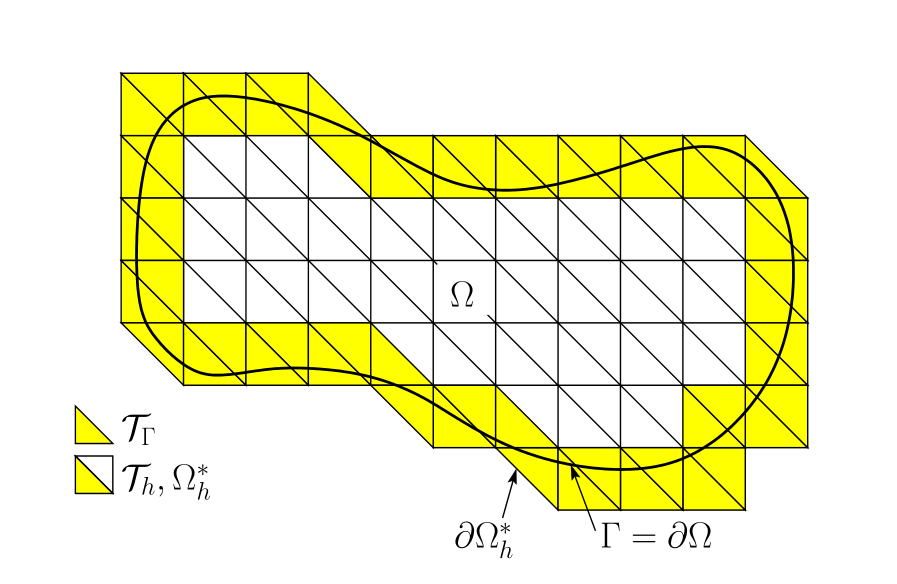
\includegraphics[width=8.2cm]{figures/minimal_subset.png}
        \end{figure}
        \end{column}

        \begin{column}{0.5\textwidth}
        \begin{block}{Observation}
            \begin{enumerate}
                \item The interior is pretty nice to deal with.
                \item The boundary must be parametrized somehow.
                    \begin{itemize}
                        \item Level-set functions $\varphi ( x) = 0 $ is one way.
                        \item Splines is also possible
                    \end{itemize}
                \item How do we deal with Dirichlet conditions?
                \item How do we deal with elements with "bad" cuts?
                \item Can we show that the problem is still well-posed?
            \end{enumerate}
        \end{block}
        \end{column}
        \end{columns}

\end{frame}

\begin{frame}{Recall Poisson problem }
        Recall the formulation \( ( \nabla u, \nabla v)_\Omega - ( \partial _{n} u, v)_{\Gamma } = ( f,v)_{\Omega }
        \)
        \begin{block}{Problem}
            \begin{itemize}
                \item
            Dirichlet conditions is embedded in the function space, \( V_{g} = \left\{ v \in H^{1 }( \Omega )   \mid  u = g \text{ on }  \Gamma   \right\} \)
        \item But is difficult to handle when $\Gamma $ is smooth.
            \end{itemize}
        \end{block}

        \begin{block}{Can we impose the Dirichlet conditions naturally?}
            Yes! We add a penalty on the boundary $ \mu (u-g,v )_{\Gamma }  $,
            \[
            ( \nabla u, \nabla v)_\Omega - ( \partial _{n} u, v)_{\Gamma }+ \mu (u,v )_{\Gamma } = ( f,v)_\Omega  + \mu (g,v )_{\Gamma }.
            \]
            For symmetry we can also add $(u-g , \partial _{n} v)_{\Gamma } $,\[
            ( \nabla u, \nabla v)_\Omega - ( \partial _{n} u, v)_{\Gamma } + (-u , \partial _{n} v)_{\Gamma }+ \mu (u,v )_{\Gamma } = ( f,v)_\Omega  + \mu (g,v )_{\Gamma }+ (-g , \partial _{n} v)_{\Gamma }.
            \]

        \end{block}
\end{frame}
\begin{frame}{Poisson formulation on a smooth boundary   }

    Recall that $\mathcal{T}_{h} $ is the active mesh, that is, all trianges intersection with the interior of the domain $\Omega$.
        \begin{block}{Definitions}
            Let $V_{h} := \mathcal{P}^{k}( \mathcal{T}_{h} )\cap C^{0}( \Omega )   $.We denote the bilinear form  $a_{h}:V_{h} \times V_{h} \to \mathbb{R} $ and the linear form  $l_{h}: V_{h} \to \mathbb{R} $ to be,\[
                \begin{split}
                a_{h}( u,v)&  :=  ( \nabla u, \nabla v)_\Omega - ( \partial _{n} u, v)_{\Gamma } - (u , \partial _{n} v)_{\Gamma }+ \mu (u,v )_{\Gamma }  \\
                l_{h} ( v) & :=( f,v)_\Omega  + \mu (g,v )_{\Gamma } - (g , \partial _{n} v)_{\Gamma }
                \end{split}
            \]

        \end{block}
        \begin{block}{Problem Statement}
            We want to find a $u \in V_{h} $ s.t. $a_{h}( u,v) = l_{h}( v)  \quad \forall v \in V_{h} $.
        \end{block}
\end{frame}

\begin{frame}{ Recall Lax Milgram }

    \begin{theorem}[ ]

        $a_{h}( u,v) = l_{h}( v)  $ well-posed if both of these statements holds;
        \begin{itemize}
            \item The bilinear form is bounded,
                \[
                      \abs{a_{h}( v,w)  }    \le C_{1} \| v \|_{a_{h}  }^{  }  \| w \|_{a_{h}  }^{  } \quad \forall v,w  \in V_{h}.
                \]
            \item The bilinear form is coercive (one-to-one), \[
           a_{h}( v,v) \ge  C_{2} \| v \|_{ a_{h} }^{  2} \quad \forall v \in V_{h}.
            \]
        \end{itemize}
    \end{theorem}
\end{frame}

\begin{frame}{Is the new system well-posed?  }

    \begin{itemize}
        \item The Dirchlet conditions problem is in good shape for smooth domains!
        \item But from basic FEM theory it is now necessarry to apply  \[
h^{\frac{1}{2}} \| \partial _{n} v \|_{ \Gamma \cap T  }^{  } \le C \| v  \|_{ \Omega \cap T      }^{  }
        \]
        to obtain well-posedness!
        \item But what about integration on very bad cut elements?
            \begin{itemize}
                \item The relation between length $  \abs{F\cap \Omega  } $ and volume $ \abs{T\cap \Omega  } $ is very different on cut elements, thus, the norm is unbounded if the cut is bad.
            \end{itemize}
    \end{itemize}

\end{frame}


\begin{frame}{The problem with the bad cuts}
        \begin{columns}
        \begin{column}{0.5\textwidth}
    \begin{figure}
        \centering
        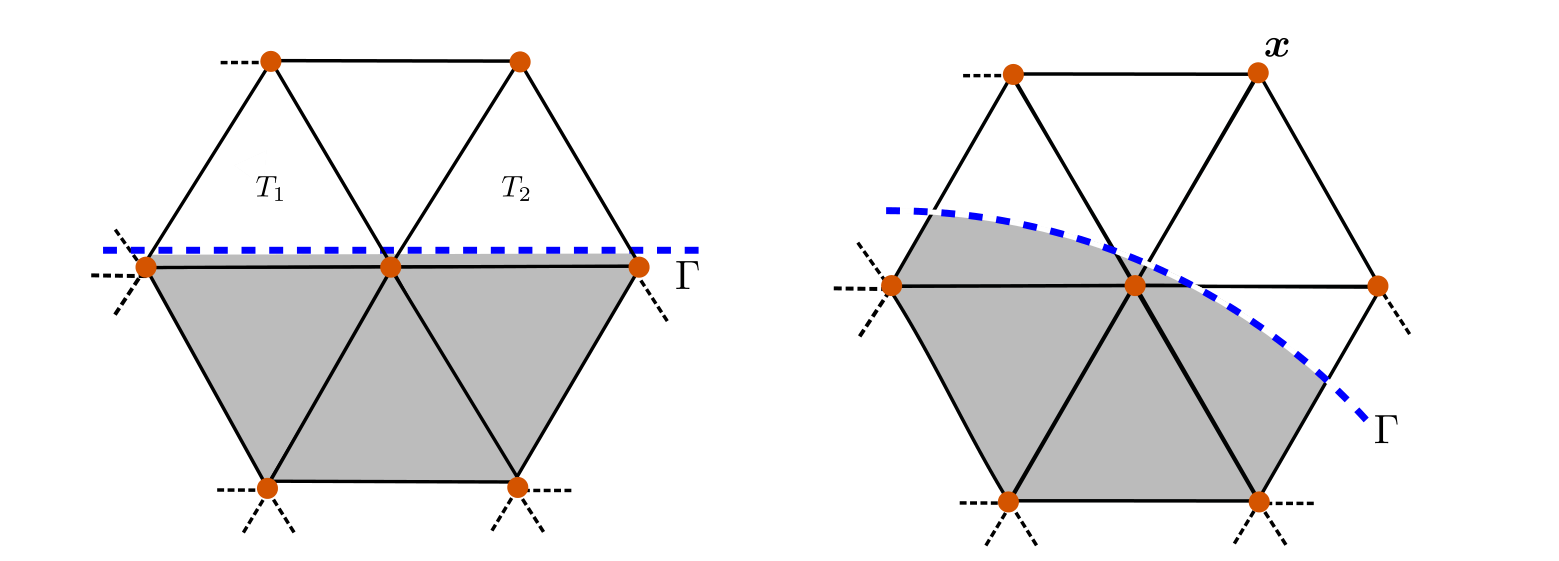
\includegraphics[width=8.8cm]{figures/bad_cuts.png}
    \end{figure}
        \end{column}

        \begin{column}{0.5\textwidth}
    \begin{block}{Observation}
        \begin{itemize}
            \item Bad cuts makes it hard to justify length $F\cap \Omega$  vs area $\abs{T\cap \Omega } $. Thus, the necessarry \[
h^{\frac{1}{2}} \| \partial _{n} v \|_{ \Gamma \cap T  }^{  } \le C \| v  \|_{ \Omega \cap T      }^{  }
            \]
            become unbounded. Hence, the system is ill-conditoned.
            \item  We are forced to extend the norm s.t. \[
h^{\frac{1}{2}} \| \partial _{n} v \|_{ \Gamma \cap T  }^{  } \le C \| v  \|_{  T      }^{  }
            \]
            But we are integrating outside of our domain :(

        \end{itemize}
    \end{block}
        \end{column}
        \end{columns}
\end{frame}

\begin{frame}{Ghost penalty}

    The solution of the inverse estimate problem is simple! We add a \textbf{ghost penalty} $g_{h}( u,v) $ to handle the bad cuts as an regularization!
    $$h^{\frac{1}{2}} \| \partial _{n} v \|_{ \Gamma \cap T  }^{  } \le C \| v  \|_{  T      }^{  }+ g_{h}( u,v) $$
    The goal is to regulate the ill-conditioned problem!
    \begin{itemize}
        \item We give it the necessarry assumptions for Lax-Milgram to hold!
        \item Same strategy is used to to obtain optimal convergence!
        \item We then engineer the $g_{h}$ given the assumptions!
    \end{itemize}

    Hence, we end up with this stabilized problem formulation

    \begin{block}{Stabilized Poission Problem}
        Let $A_{h}( u,v) := a_{h}( u,v) + g_{h}( u,v)   $.
            We want to find a $u \in V_{h} $ s.t.
            \[
            A_{h}( u,v) = l_{h}( v)  \quad \forall v \in V_{h}
            \]
    \end{block}
\end{frame}

\begin{frame}{ The reality is more nasty}

    \begin{figure}
        \centering
        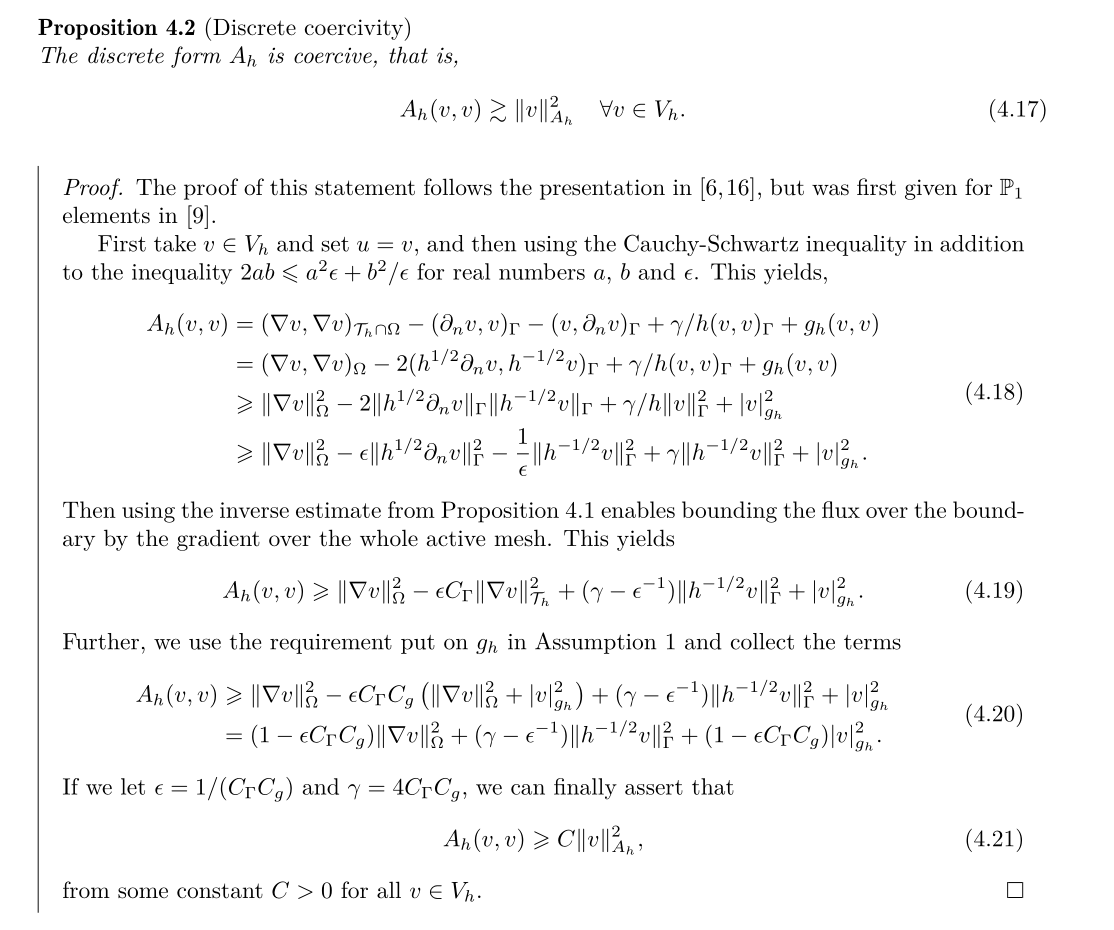
\includegraphics[width=8.5cm]{figures/reality.png}
    \end{figure}

\end{frame}
\begin{frame}{ }

    \begin{block}{But I hope at least you have learned something new :) }
    \end{block}

\end{frame}

\begin{frame}{ }

    \begin{block}{Questions? }
    \end{block}

\end{frame}



    % \begin{frame}{Example block}

    %     \begin{block}{Example}
    %         Rather than freely writing text in the frame, the use of blocks (such as this) is recommended.
    %         \begin{enumerate}
    %             \item https://www.overleaf.com/learn/latex/beamer
    %         \end{enumerate}
    %     \end{block}
    % \end{frame}

    \end{document}
